\begin{landscape}
 
 \chapter{Performanceanalyse}
	\label{performanceanalyse} 
	
	
	\section{Testgeräte}
	\begin{tabularx}{1.4\textwidth}{|l|XXX|}
		\hline
		\textbf{Abbildung} & \textbf{Gerät} & \textbf{Hardware} & \textbf{Software}\\
		\hline
		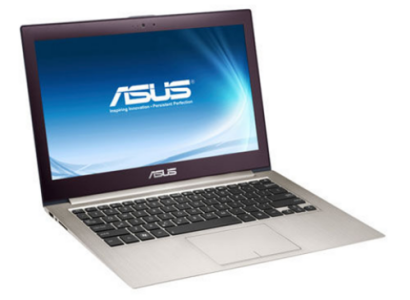
\includegraphics[width=3cm]{../performanceAnalaysis/devices/asusux21.png} & Ultrabook, Asus UX 31 & Intel Core i7 2x 1.8 GHz, 3.8GiB Memory
& Ubuntu 12.04 64Bit, Browser: Firefox 25 \\
		\hline
		
\includegraphics[width=3cm]{../performanceAnalaysis/devices/samsungnc10.jpg} & Netbook, Samsung NC 10 & Intel Atom 1.6 GHz, 992MiB Memory & Ubuntu 12.10 32Bit, Browser: Firefox 23 \\
		\hline
		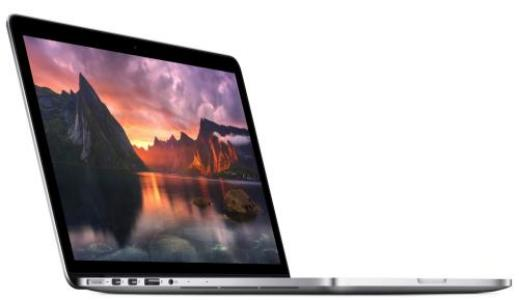
\includegraphics[width=3cm]{../performanceAnalaysis/devices/macbookpro.jpg} & Mac Book Pro 2012 & Intel Core i7 4x 2.3 GHz, 16GB Memory & Mac OS X 10.9 Mavericks, Firefox 24 \\
		\hline
		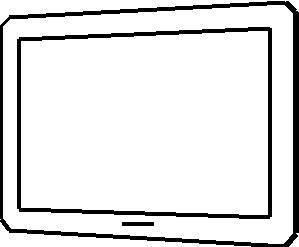
\includegraphics[width=3cm]{../performanceAnalaysis/devices/samsunggalaxy101.jpg} & Tablet, Samsung Galaxy Tab 10.1 & Nvidia Tegra 2x 1 GHz, 1GB Memory & Android 4.2.1 32 Bit, Firefox 25 \\
		\hline
		
\includegraphics[width=3cm]{../performanceAnalaysis/devices/googlenexus4.jpg} & Smartphone, Google Nexus 4 & NQualcomm Snapdragon S4 Pro 2x 1.5 GHz, 2GB Memory & Android 4.3 32 Bit, Firefox 25 \\
		\hline
	\end{tabularx}
	
	
	\section{Testszenarien und Ergebnisse}
		Die Tests wurden Bott-Up durchgeführt. Beginnend mit einem Verbindungstest zwischen zwei Browsertabs auf dem gleichen Rechner bis zu einem Test zwischen einem Client im Kabelnetz und einem Client im Mobilfunknetz.
	
		\subsection{Local Round}
			\begin{tabularx}{1.4\textwidth}{|lXX|}
				\hline
				\textbf{Geräte} & \textbf{Setup} & \textbf{Ergebnisse} \\
				\hline
					Ultrabook - Ultrabook
				&
					• 1 Browser\newline 
					• Sender und Empfänger Instanz laufen jeweils in einem Browsertab\newline 
					• Datenverkehr macht roundtripp über Netzwerkkarte\newline 
					• Externe Services wie STUN Service und Signalling Channel
				& 
					• Zunahme CPU Auslastung mit einem Channel: ca 20\%\newline
					• Zunahme Memory Verbrauch: ca 1-2\%\newline
					• Zunahme Netzwerk Trafic: keine da local loop\newline
					• Video Qualität: flüssig, genügend Frames für angenehme Bewegungsdarstellung\newline
					• Die Übertragung wird sauber beendet, keine weitere Leistungsaufnahme sobald der Stream beendet wird.\\
				\hline
			\end{tabularx}
	
			\begin{figure}[H]
				\begin{minipage}[b]{0.5\linewidth}
					\centering
					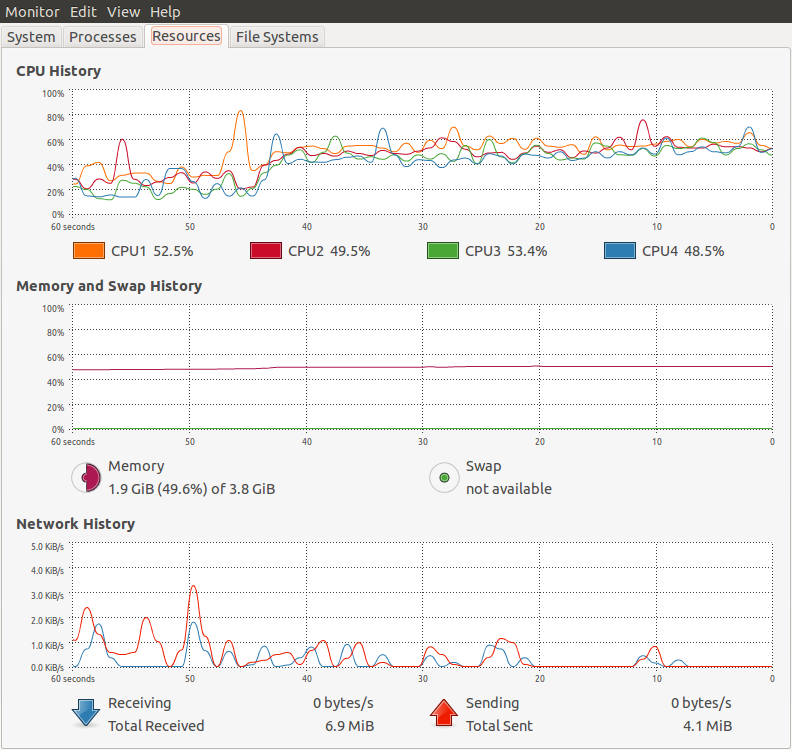
\includegraphics[width=\linewidth]{{../performanceAnalaysis/img/messung1.2.1.1}.png}
					\caption{CPU Leistung für einen Stream}
				\end{minipage}		
				\begin{minipage}[b]{0.5\linewidth}
					\centering
					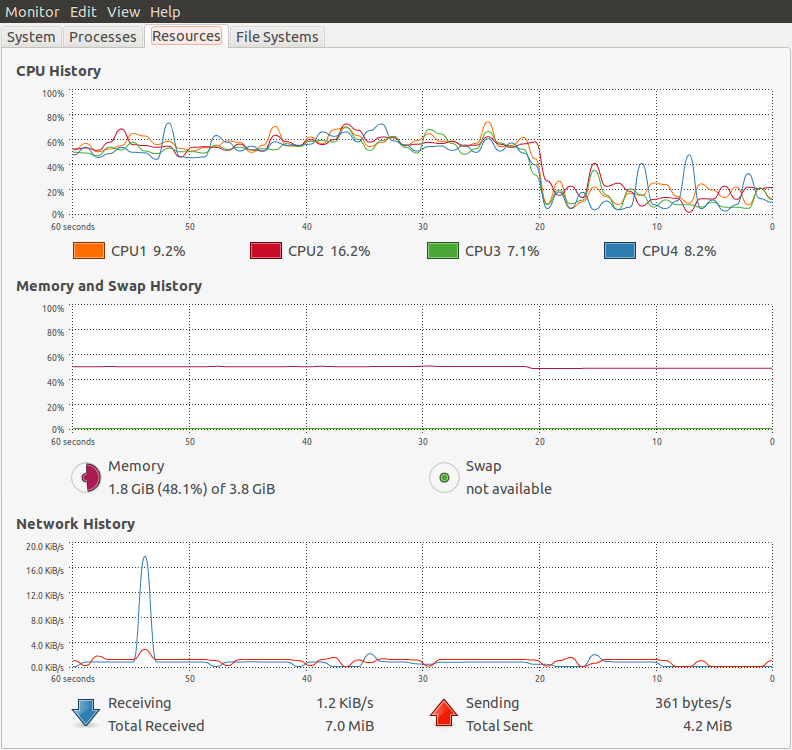
\includegraphics[width=\linewidth]{{../performanceAnalaysis/img/messung1.2.1.2}.png}
					\caption{Vollständige Rückgabe der CPU an andere Prozesse nach dem Ende der Übertragung}
				\end{minipage}
			\end{figure}
			
			
		\subsection{Remote}
			\begin{tabularx}{1.4\textwidth}{|lXX|}
				\hline
				\textbf{Geräte} & \textbf{Setup} & \textbf{Ergebnisse} \\
				\hline
					Ultrabook - Netbook
				&
					• 1 Ultrabook, 1 Netbook\newline 
					• Jeweils gleicher Browser\newline 
					• Datenverkehr läuft über HSR Wlan
				& 
					\textbf{Netbook}:\newline
					• Zunahme CPU Auslastung: ca 50\%\newline
					• Zunahme Memory Verbrauch: nicht spürbar\newline
					• Zunahme Netzwerk Trafic: 10KiB/s out, 15KiB/s\newline
					\textbf{Qualität}: \newline
					• stockend, wenige Frames/s, unbrauchbar für Bewegungsdarstellung\newline
					• Audio Qualität: unbrauchbar\newline
					• Zunahme Netzwerk Trafic: 10KiB/s out, 15KiB/s\\
				\hline				
			\end{tabularx}
			\begin{figure}[H]
				\centering
				\begin{minipage}[b]{0.5\linewidth}
					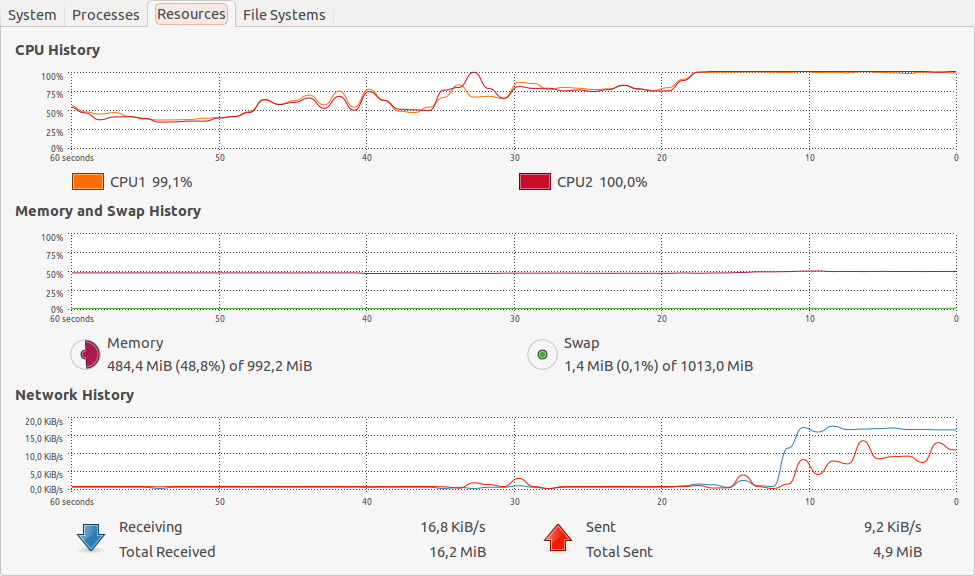
\includegraphics[width=\linewidth]{{../performanceAnalaysis/img/messung2.2.1.1}.png}
					\caption{Das Netbook ist bis an die Leistungsgrenze ausgelastet}
				\end{minipage}
			\end{figure}
			
			
			\begin{tabularx}{1.4\textwidth}{|lXX|}
				\hline
				\textbf{Geräte} & \textbf{Setup} & \textbf{Ergebnisse} \\
				\hline
					Ultrabook - Netbook
				&
					• Gleich wie bei vorherigem Versuch\newline
					• Nur Audio, keine Videoübertragung
				& 
					\textbf{Netbook}:\newline
					• Zunahme CPU Auslastung: ca 20\%\newline
					• Zunahme Memory Verbrauch: nicht spürbar\newline
					• Zunahme Netzwerk Trafic: 7KiB/s in/out\newline
					\textbf{Ultrabook}:\newline
					• Zunahme CPU Auslastung: ca. 10\%\newline
					• Zunahme Memory Verbrauch: nicht spürbar\newline
					• Zunahme Netzwerk Trafic: 8 KiB/s out, 7KiB/s in, Abbruch des Streams nach 30s\\
				\hline				
			\end{tabularx}
			\begin{figure}[H]
				\begin{minipage}[b]{0.5\linewidth}
					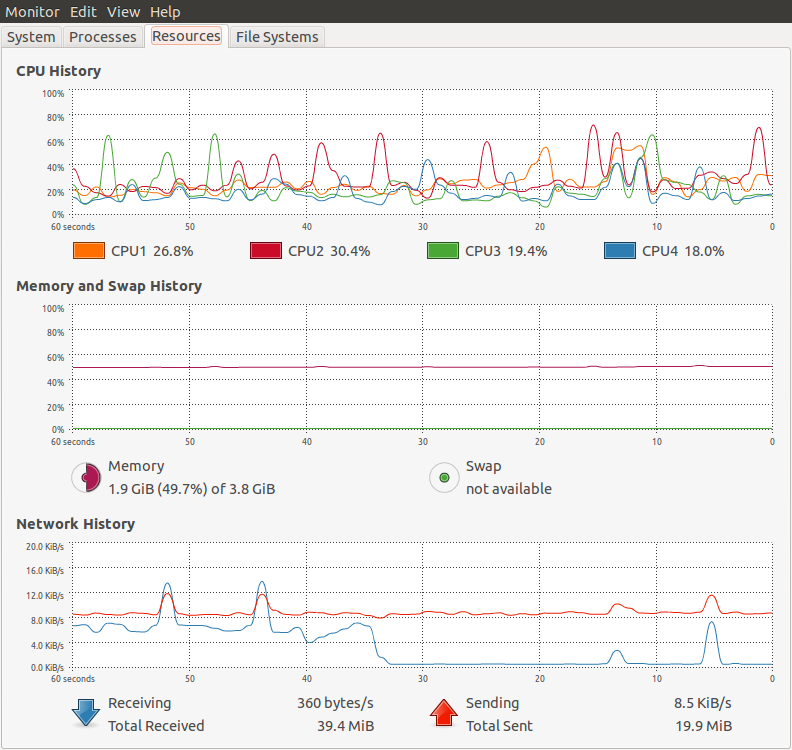
\includegraphics[width=\linewidth]{{../performanceAnalaysis/img/messung2.2.2.1}.png}
					\caption{CPU Belastung Ultrabook}
				\end{minipage}
				\begin{minipage}[b]{0.5\linewidth}
					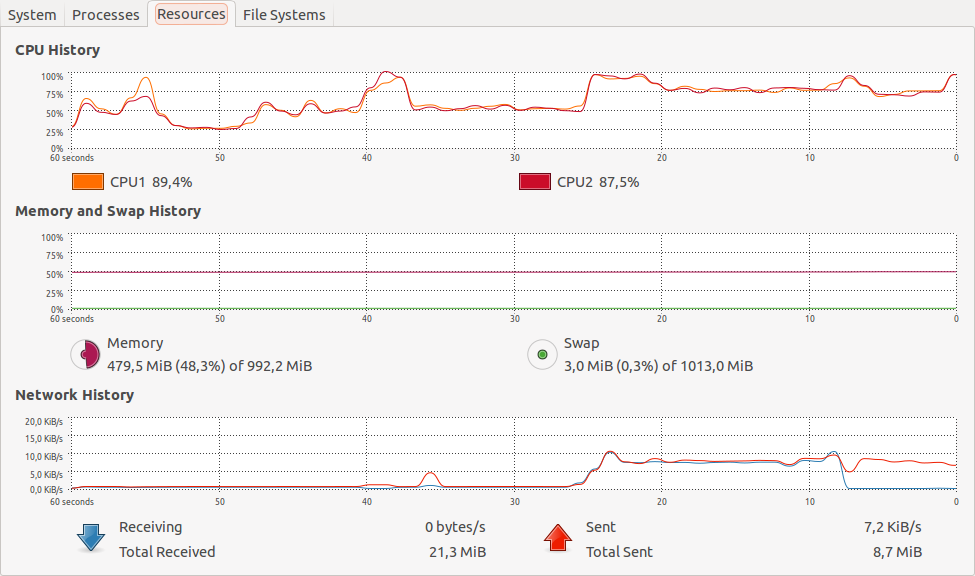
\includegraphics[width=\linewidth]{{../performanceAnalaysis/img/messung2.2.2.2}.png}
					\caption{CPU Belastung Netbook}
				\end{minipage}
			\end{figure}
	
	
			\begin{tabularx}{1.4\textwidth}{|lXX|}
				\hline
				\textbf{Geräte} & \textbf{Setup} & \textbf{Ergebnisse} \\
				\hline
					Ultrabook - Mac Book
				&
					• 1 Ultrabook, 1 Macbook\newline
					• Jeweils gleicher Browser\newline
					• Datenverkehr läuft über HSR Wlan
				& 
					\textbf{Ultrabook}:\newline
					• Zunahme CPU Auslastung: ca 20\%\newline
					• Zunahme Memory Verbrauch: nicht spürbar\newline
					• Zunahme Netzwerk Trafic: 50KiB/s, steigend bis 150KiB/s\newline
					\textbf{Qualität}:\newline
					• Flüssige Audio- und Video Übertragung in beide Richtungen\newline
					• Stream des Macbook's sind keine Einzelbilder sichtbar\newline
					• Stream des Ultrabooks zeigt bei schnellen Bewegungen Einzelbilder\newline
					• Gut geeignet für Bewegungsdarstellung\\
				\hline				
			\end{tabularx}
			\begin{figure}[H]
				\centering
				\begin{minipage}[b]{0.5\linewidth}
					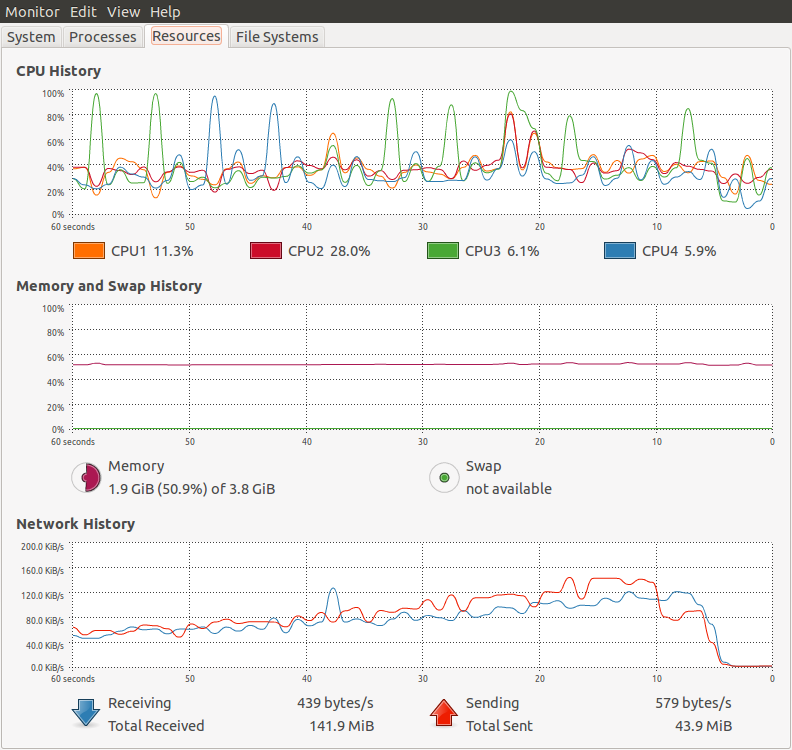
\includegraphics[width=\linewidth]{{../performanceAnalaysis/img/messung2.3.1}.png}
					\caption{Ansteigende (automatisch skalierende) Datenrate, da beide Geräte entsprechende Videoauflösungen liefern können}
				\end{minipage}
			\end{figure}
			
			
		\subsection{Mobile - Desktop}
			\begin{tabularx}{1.4\textwidth}{|lXX|}
				\hline
				\textbf{Geräte} & \textbf{Setup} & \textbf{Ergebnisse} \\
				\hline
					Ultrabook - Tablet
				&
					• 1 Ultrabook, 1 Tablet\newline
					• Beide Geräte im HSR Wlan
				& 
					\textbf{Tablet}:\newline
					• Zunahme CPU Auslastung: ca 70\%\newline
					\textbf{Qualität}:\newline
					• Tablet kann Video vom Desktop flüssig wiedergeben, auch der Ton wird korrekt und verständlich wiedergegeben\newline
					• Tablet bringt Leistung nicht um eigenes Video parallel zum remote zu verarbeiten -> eigenes Video freezed\newline
					• Desktop empfängt entsprechend vom Tablet nur ein Standbild\\
				\hline
			\end{tabularx}\newline
			
			\noindent
			\begin{tabularx}{1.4\textwidth}{|lXX|}
				\hline
				\textbf{Geräte} & \textbf{Setup} & \textbf{Ergebnisse} \\
				\hline
					Ultrabook - Smartphone
				&
					• 1 Ultrabook, 1 Smartphone\newline
					• Beide Geräte im HSR Wlan
				& 
					\textbf{Qualität}:\newline
					• Video kann sowohl auf dem Phone wie auf dem Desktop einigermassen flüssig wiedergegeben werden\newline
					• Die video Auflösung ist relativ gering\newline
					• Geeignet für Bewegungsdarstellung\\
				\hline				
			\end{tabularx}\newline
			
			\noindent
			\begin{tabularx}{1.4\textwidth}{|lXX|}
				\hline
				\textbf{Geräte} & \textbf{Setup} & \textbf{Ergebnisse} \\
				\hline
					Ultrabook - Smartphone
				&
					• 1 Ultrabook, 1 Smartphone\newline
					• Gleiches Setup wie bei vorherigem Versuch
				& 
					\textbf{Qualität}:\newline
					• Wird das Smartphone gedreht, so verändert die Kamera die Auflösung und refreshed den Stream.\newline
					• Der Stream wird jeweils neu aufgebaut. Dabei wird er auf 40KiB/s gedrosselt und langsam
hochgefahren.\newline
					• Dieses automatische Quality Scaling funktioniert nur, wenn das Gerät dies unterstützt.\newline
					• Das Smartphone wird während der Kommunikation ziemlich warm und warnt bald vor schrumpfender
Akkuleistung.\\
				\hline				
			\end{tabularx}
			\begin{figure}[H]
				\begin{minipage}[b]{0.5\linewidth}
					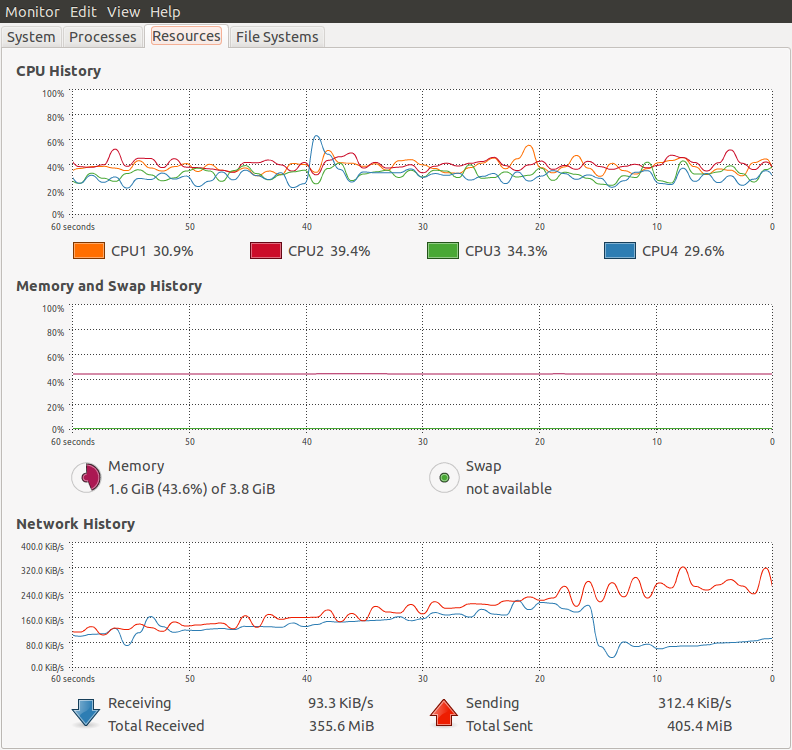
\includegraphics[width=\linewidth]{{../performanceAnalaysis/img/messung3.3.1}.png}
					\caption{Zur Sekunde 25 wird das Smartphone von Widescreen Ausrichtung nach Portrait gedreht. Dabei wird die Datenrate auf das bereits mehrfach beobachtete minimum von 40KiB/s gedrosselt und anschliessend langsam hochgefahren.}
				\end{minipage}
				\begin{minipage}[b]{0.5\linewidth}
					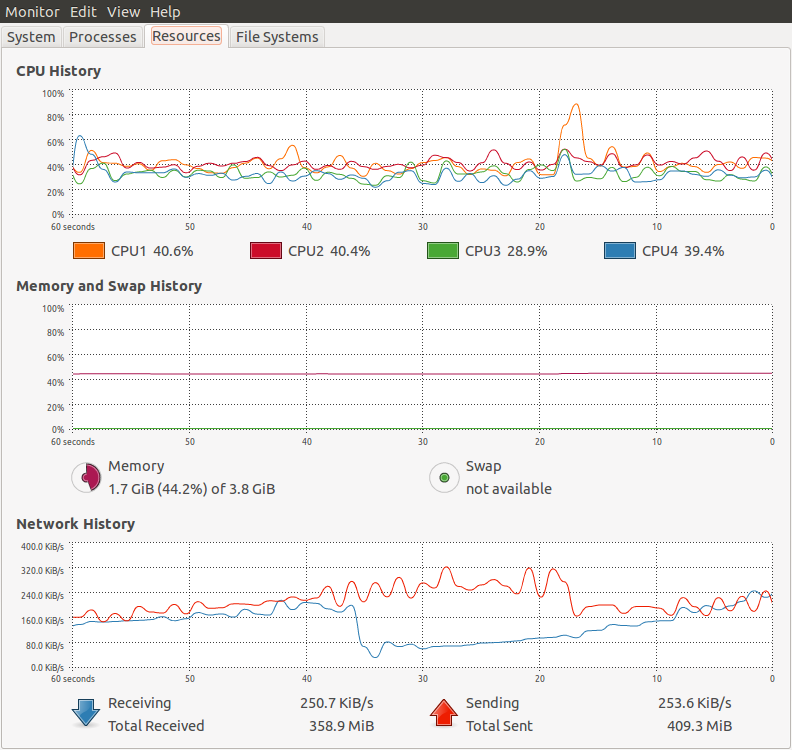
\includegraphics[width=\linewidth]{{../performanceAnalaysis/img/messung3.3.2}.png}
					\caption{Die Datenrate wird bis auf 300KiB/s hochgefahren, wenn die Geräte dies liefern können. Zur 15. Sekunde findet eine Neuausrichtung des Smartphones statt.}
				\end{minipage}
			\end{figure}
			\begin{figure}[H]
				\begin{minipage}[b]{0.5\linewidth}
					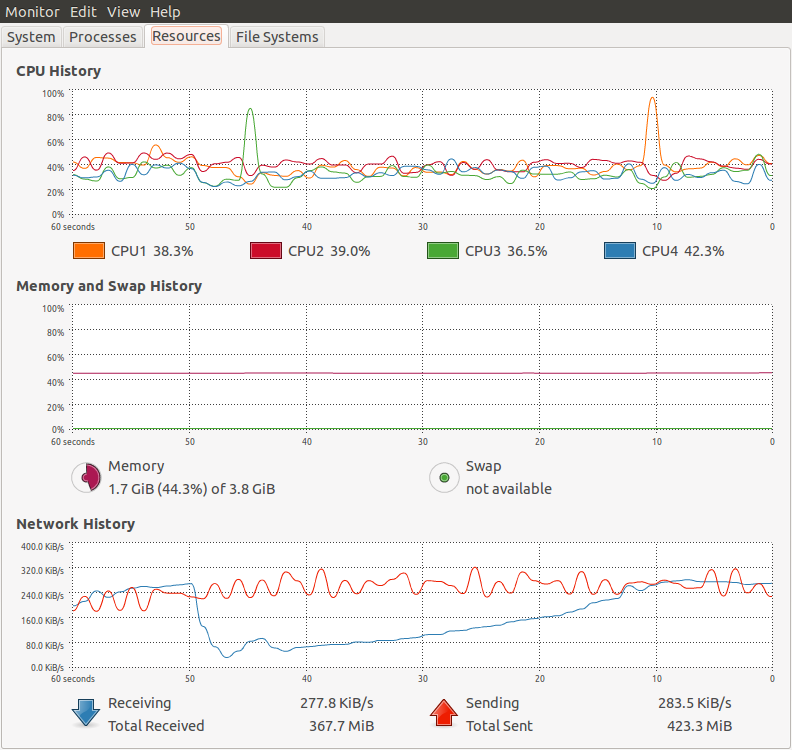
\includegraphics[width=\linewidth]{{../performanceAnalaysis/img/messung3.3.3}.png}
					\caption{Drehung des Smartphone nach Widescreen. Nach 40s erreicht die Auflösung wieder die ursprüngliche Auflösung.}
				\end{minipage}
				\begin{minipage}[b]{0.5\linewidth}
					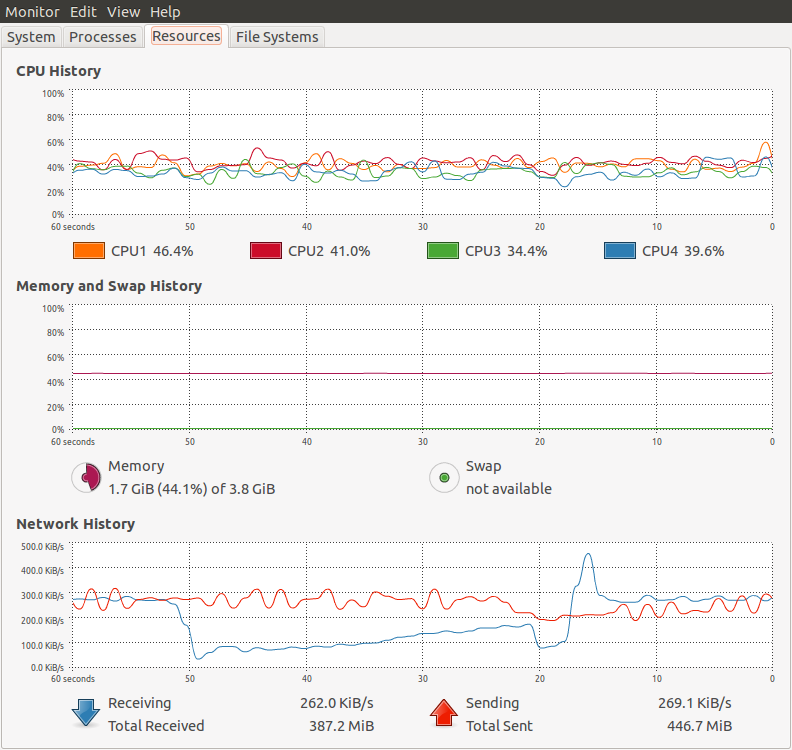
\includegraphics[width=\linewidth]{{../performanceAnalaysis/img/messung3.3.4}.png}
					\caption{Ein Kurzer Pufferunterlauf zur Sekunde 40 führt daraufhin zu einem Peak. Anschliessend pendelt sich die Datenrate bei 300 KiB/s ein.}
				\end{minipage}
			\end{figure}
			
			
		\subsection{Out of Network}
			\begin{tabularx}{1.4\textwidth}{|lXX|}
				\hline
				\textbf{Geräte} & \textbf{Setup} & \textbf{Ergebnisse} \\
				\hline
					Ultrabook - Smartphone
				&
					• 1 Ultrabook, 1 Smartphone\newline
					• Smartphone direkt über Home Wlan angebunden\newline
					• Ultrabook über Home Wlan mit HSR VPN angebunden
				& 
					\textbf{Ultrabook}:\newline
					• Zunahme CPU Auslastung: ca 20\%\newline
					• Zunahme Memory Verbrauch: nicht spürbar\newline
					• Zunahme Netzwerk Trafic: 1-5KiB/s\newline
					• Sprache gut unverständlich\newline
					\textbf{Qualität}:\newline
					• Video stockend oder flüssig, je nach dem ob die Pakete gut durchkommen oder nicht.\newline
					• Smartphone wird etwas warm\newline
					• Video Verzögerung von bis zu ca. 4s\newline
					• Sprache verständlich oder unverständlich, je nach dem wie gut die Übertragungsrate ist.\\
				\hline				
			\end{tabularx}
				\centering
				\begin{minipage}[b]{0.5\linewidth}
					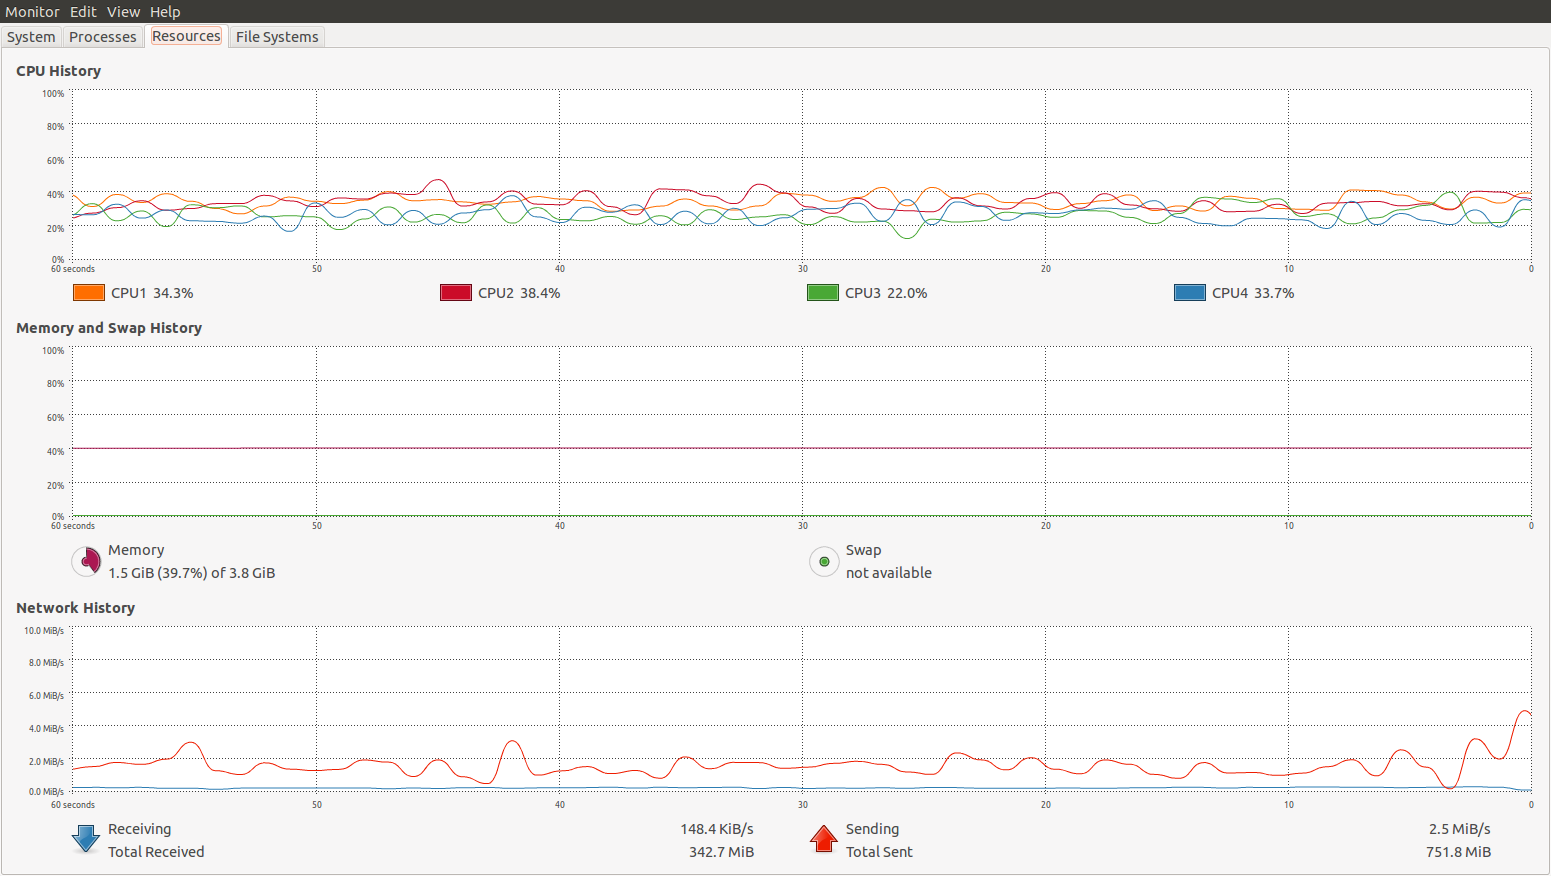
\includegraphics[width=\linewidth]{{../performanceAnalaysis/img/messung4.1.1}.png}
					\caption{Das Ultrabook kann einige wenige KiB/s liefern, das Smartphone sogar nut 1KiB/s.}
				\end{minipage}
			\end{figure}			
			\begin{figure}[H]
				\begin{minipage}[b]{0.5\linewidth}
					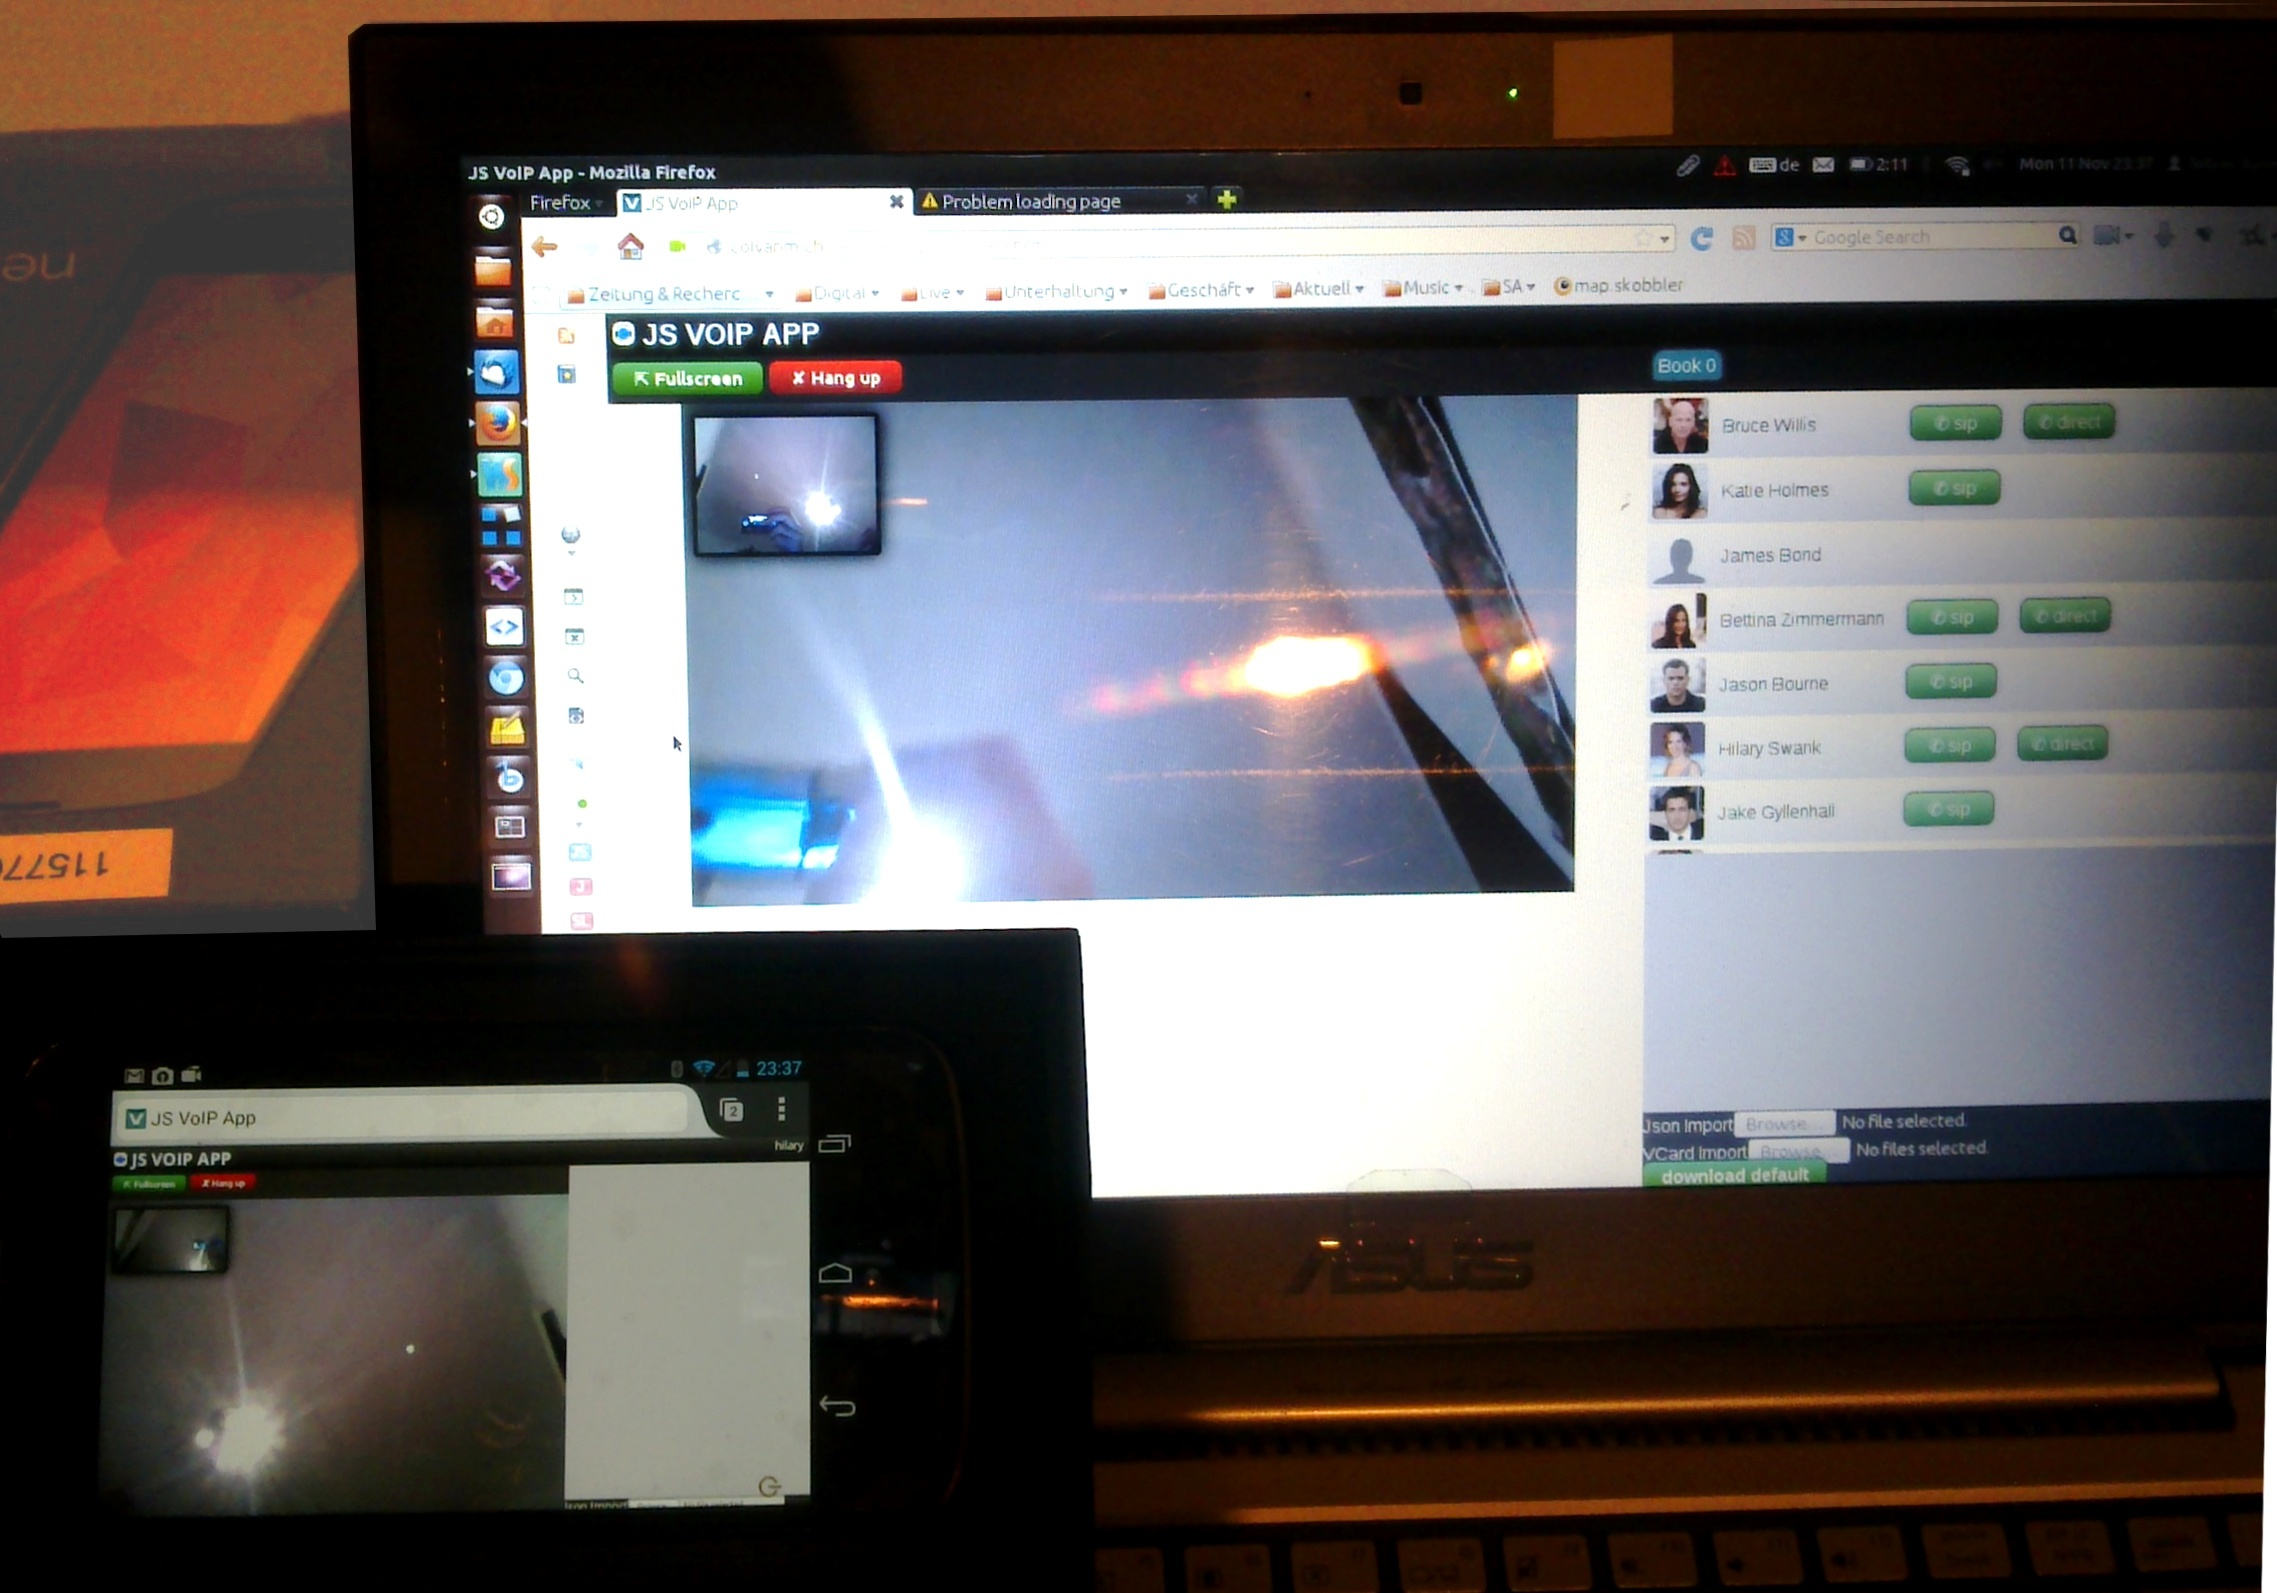
\includegraphics[width=\linewidth]{{../performanceAnalaysis/img/messung4.1.3.1}.jpg}
					\caption{Videokommunikation zwischen Smartphone und Ultrabook}
				\end{minipage}
				\begin{minipage}[b]{0.5\linewidth}
					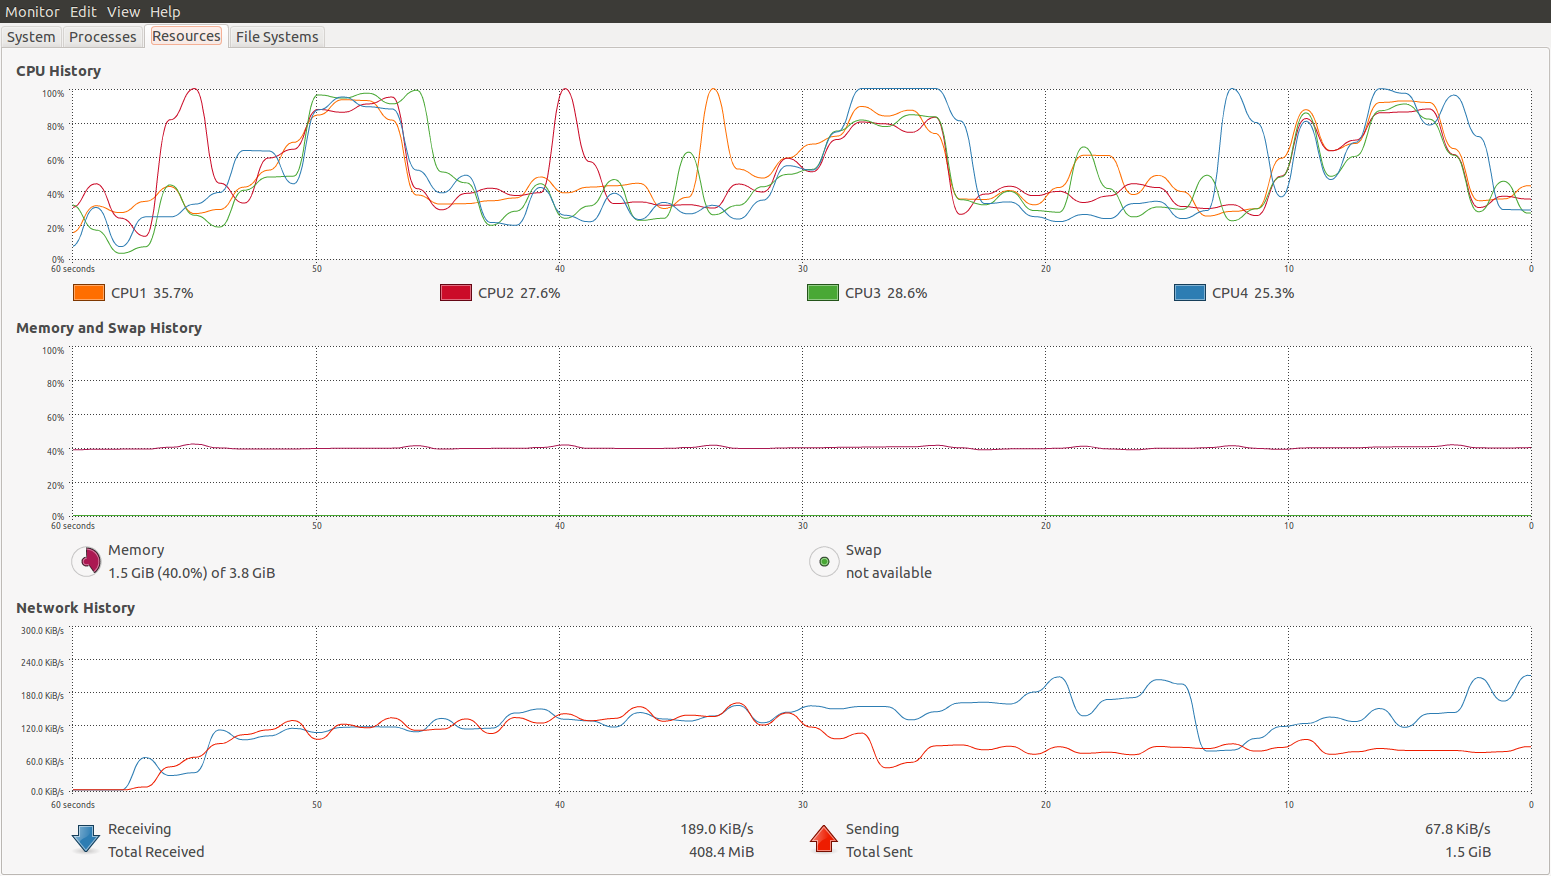
\includegraphics[width=\linewidth]{{../performanceAnalaysis/img/messung4.1.2}.png}
					\caption{Die Datenrate fährt hoch bis über 100 KiB/s. Drehung des Smartphones zur Sekunde 55}
				\end{minipage}
			\end{figure}
			
		\subsection{Festnetz - Mobilfunknetz}
			\begin{tabularx}{1.4\textwidth}{|lXX|}
				\hline
				\textbf{Geräte} & \textbf{Setup} & \textbf{Ergebnisse} \\
				\hline
					Ultrabook - Netbook
				&
					• 1 Ultrabook, 1 Netbook\newline
					• Netbook über UMTS (Stadt) angebunden\newline
					• Ultrabook über Home Wlan angebunden\newline
					• 1. Mal Video+Audio, 2. Mal nur Audio
				& 	
					\textbf{Ultrabook}:\newline
					• Zunahme Netzwerk Trafic bei Video: ca32-70KiB/s\newline
					• Zunahme Netzwerk Trafic bei Audio: ca8KiB/s\newline
					\textbf{Qualität (Video)}:\newline
					• Video stockend\newline
					• Audio verzögert und nur knapp verständlich\newline
					\textbf{Qualität (nur Audio)}:\newline
					• Audio flüssig, kaum verzögert und gut verständlich\\
				\hline	
			\end{tabularx}
			\begin{figure}[H]
				\begin{minipage}[b]{0.5\linewidth}
					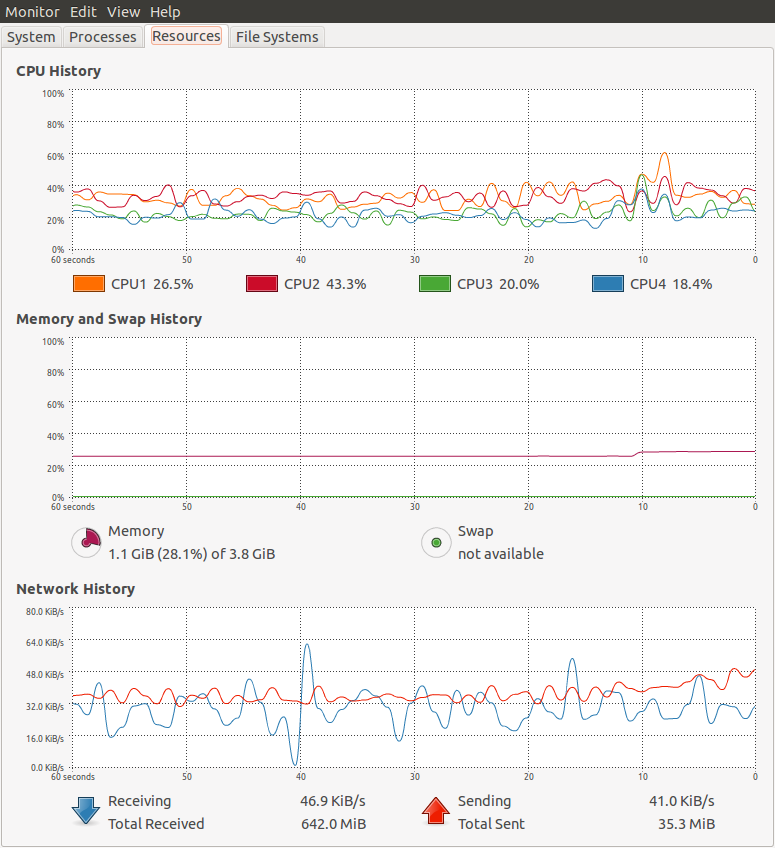
\includegraphics[width=\linewidth]{{../performanceAnalaysis/img/messung5.1.1}.png}
					\caption{Ultrabook: Die Videowiedergabe ist nach dem Start noch relativ schmalbandig}
				\end{minipage}
				\begin{minipage}[b]{0.5\linewidth}
					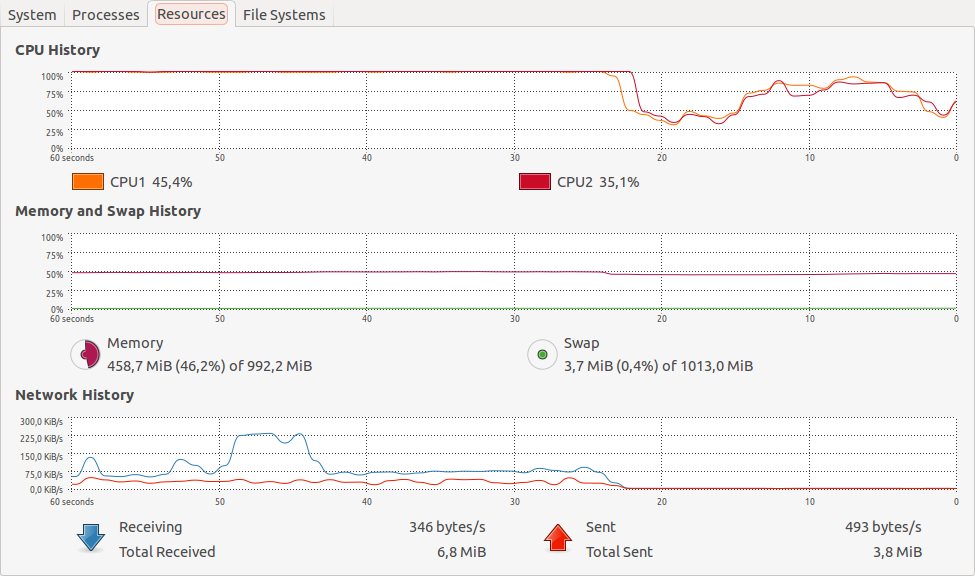
\includegraphics[width=\linewidth]{{../performanceAnalaysis/img/messung5.1.2}.png}
					\caption{Netbook: Die Datenrate vom Ultrabook ist etwas höher als die des Netbook.}
				\end{minipage}
			\end{figure}			
			\begin{figure}[H]
				\begin{minipage}[b]{0.5\linewidth}
					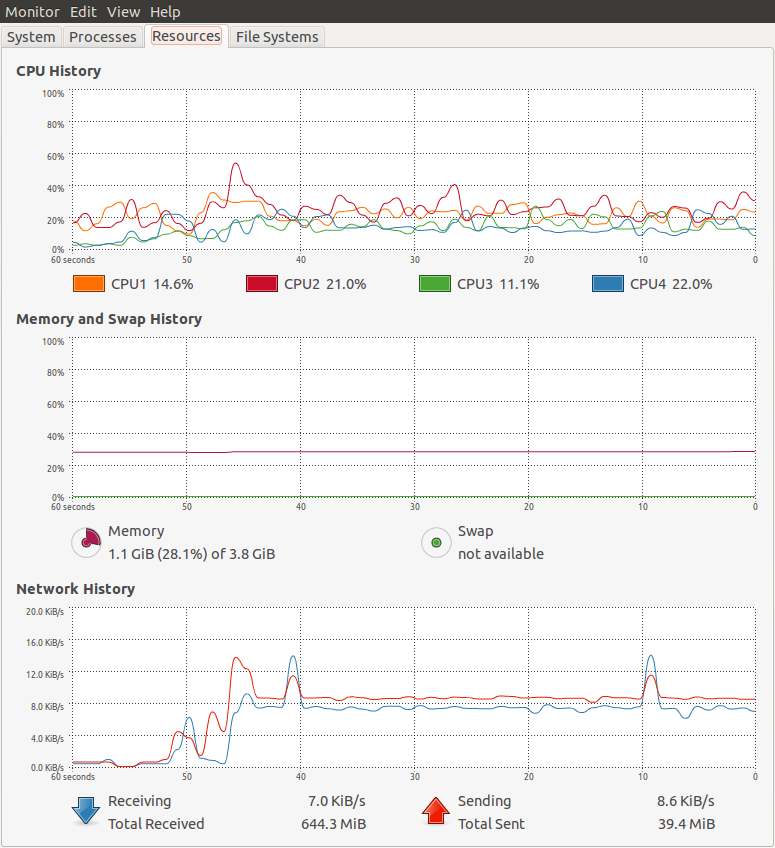
\includegraphics[width=\linewidth]{{../performanceAnalaysis/img/messung5.1.3}.png}
					\caption{Ultrabook: Audiodatenrate nach dem Verbinden}
				\end{minipage}
				\begin{minipage}[b]{0.5\linewidth}
					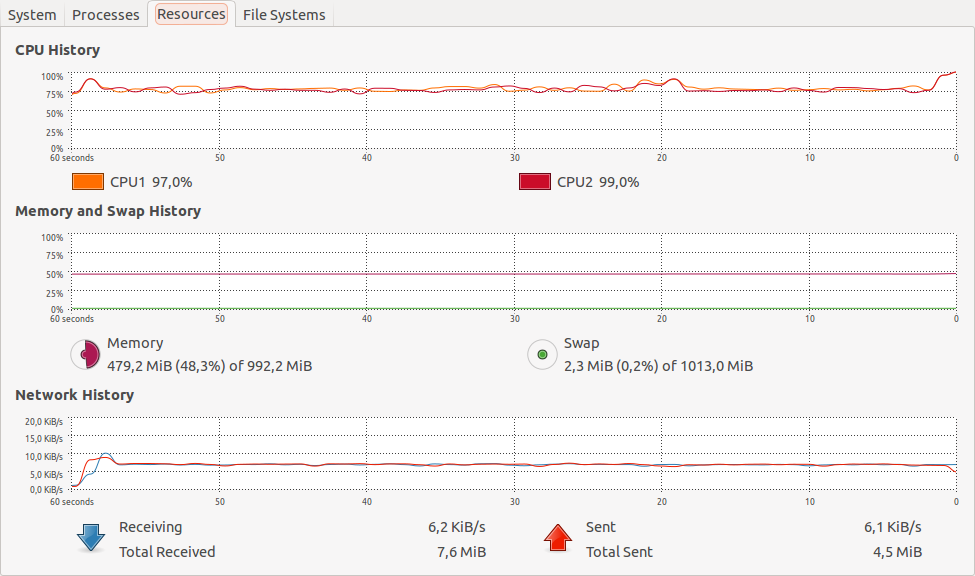
\includegraphics[width=\linewidth]{{../performanceAnalaysis/img/messung5.1.4}.png}
					\caption{Netbook: Audiodatenrate nach einiger Zeit (eingependelt)}
				\end{minipage}
			\end{figure}	
	
\end{landscape}
	
	